\documentclass[12pt,a4paper]{article}
\usepackage{pgf}
\usepackage{svg}
\usepackage{tikz}
\usepackage{stanli}
\usepackage{afterpage}
\usepackage{multirow}
\usepackage{subfig}
\usepackage{pgfpages}
\usepackage{svg}
\usepackage{rotating}
\usepackage{algorithm}
\usepackage{algpseudocode}
\pgfpagesdeclarelayout{boxed}{
	\edef\pgfpageoptionborder{0pt}
}{
	\pgfpagesphysicalpageoptions
	{%
		logical pages=1,%
	}
	\pgfpageslogicalpageoptions{1}
	{
		border code=\pgfsetlinewidth{2pt}\pgfstroke,%
		border shrink=\pgfpageoptionborder,%
		resized width=.9\pgfphysicalwidth,%
		resized height=.9\pgfphysicalheight,%
		center=\pgfpoint{.5\pgfphysicalwidth}{.5\pgfphysicalheight}%
	}%
}

\pgfpagesuselayout{boxed}


% Language setting
% Replace `english' with e.g. `spanish' to change the document language
\usepackage[english]{babel}

% Set page size and margins
% Replace `letterpaper' with `a4paper' for UK/EU standard size
\usepackage[a4paper,top=2cm,bottom=1.5cm,left=1.5cm,right=1.5cm,marginparwidth=1.75cm]{geometry}

% Useful packages
\usepackage{amsmath}
\usepackage{graphicx}
\usepackage[colorlinks=true, allcolors=blue]{hyperref}

\usepackage[english]{babel}
\usepackage{microtype,etex,listings,color,parskip}
\lstset{
  language=C,
  tabsize=2,
  showstringspaces=false,
  breaklines=true,
  basicstyle=\ttfamily,
  keywordstyle=\color[rgb]{0.1,0.3,0.7}\ttfamily,
  stringstyle=\color[rgb]{0.7,0.1,0.3}\ttfamily,
  commentstyle=\color[rgb]{0.3,0.4,0.3}\ttfamily,
  columns=fixed,
  numberstyle=\sffamily\scriptsize,
  backgroundcolor=\color[rgb]{0.95,0.95,0.95},
  frame=lines,
  framexleftmargin=5pt,
  numbers = left,
  numberstyle = \footnotesize
}
% ... until here -------------------------------------------

\begin{document}
	
	\newcommand{\subf}[2]{%
		{\small\begin{tabular}[t]{@{}c@{}}
				#1\\#2
		\end{tabular}}%
	}
	
	\begin{titlepage}
		\begin{center}
			\vspace*{3cm}
			
			\Large
			\textbf{Programarea calculatoarelor si limbaje de programare}
			
			\vspace{0.3cm}
				\Large
			Sistemul de management al informațiilor angajaților
			
			\vspace{0.8cm}
			\large
			
			
			\vspace{0.5cm}
			\LARGE
			
			\vspace{1.5cm}
			
			\textbf{}
            
\includegraphics[width=0.3\textwidth]{logo-ace.jpg}
			
			\vfill
			\vspace{0.6cm}
	
			\Large
			
		\end{center}
		\Large
		\begin{tabbing}
			\hspace*{1em}\= \hspace*{8em} \= \kill % set the tabbings
			\> Nume Student 1:\>  \textbf{Torcea Ciprian-Marius} \\
                \> Nume Student 2:\>  \textbf{Văduva Alex} \\
			\> Subgrupa:\>  B \\
			\> Grupa:\>  CR 1.3 \\
			\> Profesor:  \> Asist. Univ. Alexandra Vultureanu-Albisi  \\
		\end{tabbing}
	\end{titlepage}
	
	\tableofcontents

\newpage
\section{INTRODUCERE}
\subsection{Enuntul problemei}
 
Datele angajaților trebuie păstrate în orice companie. Fiecare companie are un angajat cu un ID
unic de angajat, rol de angajat etc. Toate aceste date sunt păstrate într-un sistem de management
al angajaților, unde sunt stocate toate datele despre fiecare angajat, putem prelua, actualiza și
adăuga date la acest sistem. Folosind C putem crea un sistem de management al angajaților care
poate îndeplini toate aceste sarcini, folosind cunoștințe de bază C precum șir, matrice, fișier etc.\\\\
\textbf{Funcționalitatea Sistemului de management al angajaților este:}\\
Realizați tabelul cu angajați.\\
Inserați intrări noi.\\
Ștergeți intrările.\\
Căutați o înregistrare.

\subsection{Descrierea problemei}

Problema abordată în acest program este gestionarea informațiilor despre angajații unei companii printr-un sistem de management al angajaților.\\ Scopul principal este să ofere o interfață utilizatorului pentru a adăuga, șterge, căuta și afișa informații despre angajați. Acest sistem utilizează un set de funcționalități de bază precum afișarea, adăugarea, ștergerea și căutarea angajaților într-un tabel.\\\\
\textbf{\textit{Principalele componente ale problemei sunt:}}\\\\
\textbf{Structura de date:} Un angajat este reprezentat printr-o structură care conține un ID unic, nume și rol în cadrul companiei.\\\\
\textbf{Funcționalități principale:}\\
\begin{enumerate}
    \item Afișarea tabelului cu angajați.
    \item Adăugarea unei noi înregistrări pentru un angajat.
    \item Ștergerea unei înregistrări bazată pe ID-ul angajatului.
    \item Căutarea unui angajat în funcție de ID.
\end{enumerate}
\textbf{Persistența datelor:} \\\\
Datele despre angajați pot fi salvate și încărcate dintr-un fișier pentru a asigura persistența informațiilor între rulările programului.\\

\newpage

\section{ALGORITMI}
\subsection{Pseudocod}

\section*{Pseudocod pentru Funcția \textsc{printMenu}}
\begin{algorithm}
\begin{algorithmic}[1]
    \State Afișează textul pentru meniu
    \State Încheie funcția
\end{algorithmic}
\end{algorithm}

\section*{Pseudocod pentru Funcția \textsc{printEmployee}}
\begin{algorithm}
\begin{algorithmic}[1]
    \State Afișează informațiile despre angajat (ID, nume, rol)
    \State Încheie funcția
\end{algorithmic}
\end{algorithm}

\section*{Pseudocod pentru Funcția \textsc{addEmployee}}
\begin{algorithm}
\begin{algorithmic}[1]
    \If{count $<$ MAX\_EMPLOYEES}
        \State Afișează un mesaj de introducere
        \State Citește ID-ul, numele și rolul pentru noul angajat
        \State Incrementează count
        \State Afișează un mesaj de succes
    \Else
        \State Afișează un mesaj că numărul maxim de angajați a fost atins
    \EndIf
    \State Încheie funcția
\end{algorithmic}
\end{algorithm}

\section*{Pseudocod pentru Funcția \textsc{displayEmployees}}
\begin{algorithm}
\begin{algorithmic}[1]
    \State Afișează un antet pentru tabelul de angajați
    \ForAll{angajat în angajați}
        \State Apelează \textsc{printEmployee} cu angajatul curent
    \EndFor
    \State Afișează un separator pentru tabel
    \State Încheie funcția
\end{algorithmic}
\end{algorithm}

\newpage

\section*{Pseudocod pentru Funcția \textsc{deleteEmployee}}
\begin{algorithm}
\begin{algorithmic}[1]
    \State Inițializează index cu -1
    \ForAll{angajat în angajați}
        \If{angajatul curent are ID-ul dorit}
            \State Setează index cu indicele curent
            \State Ieșește din bucla for
        \EndIf
    \EndFor
    \If{index $\neq$ -1}
        \For{i de la index la count - 1}
            \State Copiază angajatul de la i+1 la i
        \EndFor
        \State Decrementează count
        \State Afișează un mesaj de succes
    \Else
        \State Afișează un mesaj că angajatul nu a fost găsit
    \EndIf
    \State Încheie funcția
\end{algorithmic}
\end{algorithm}

\section*{Pseudocod pentru Funcția \textsc{searchEmployee}}
\begin{algorithm}
\begin{algorithmic}[1]
    \State Inițializează found cu 0
    \ForAll{angajat în angajați}
        \If{angajatul curent are ID-ul dorit}
            \State Apelează \textsc{printEmployee} cu angajatul curent
            \State Setează found la 1
            \State Ieșește din bucla for
        \EndIf
    \EndFor
    \If{found $==$ 0}
        \State Afișează un mesaj că angajatul nu a fost găsit
    \EndIf
    \State Încheie funcția
\end{algorithmic}
\end{algorithm}

\newpage
\section*{Pseudocod pentru Funcția \textsc{saveToFile}}
\begin{algorithm}
\begin{algorithmic}[1]
    \State Deschide un fișier pentru scriere (file)
    \If{file nu există}
        \State Afișează un mesaj de eroare
        \State Încheie funcția
    \EndIf
    \ForAll{angajat în angajați}
        \State Scrie informațiile despre angajat în file
    \EndFor
    \State Închide file
    \State Afișează un mesaj de succes
    \State Încheie funcția
\end{algorithmic}
\end{algorithm}

\section*{Pseudocod pentru Funcția \textsc{loadFromFile}}
\begin{algorithm}
\begin{algorithmic}[1]
    \State Deschide un fișier pentru citire (file)
    \If{file nu există}
        \State Afișează un mesaj că fișierul nu poate fi deschis
        \State Încheie funcția
    \EndIf
    \While{se poate citi din file}
        \State Citește ID-ul, numele și rolul pentru un angajat nou
        \State Incrementează count
        \If{count $\geq$ MAX\_EMPLOYEES}
            \State Afișează un mesaj că numărul maxim de angajați a fost atins
            \State Încheie bucla while
        \EndIf
    \EndWhile
    \State Închide file
    \State Afișează un mesaj de succes
    \State Încheie funcția
\end{algorithmic}
\end{algorithm}

\subsection{Scheme Logice}
Meniul aplicației noastre de management al angajaților oferă mai multe opțiuni, iar pentru fiecare opțiune am implementat o metodă specifică, aplicația fiind modulară. \\\\
În următoare figură sunt evidențiate opțiunile disponibile ale meniului:
\begin{figure}
    \centering
    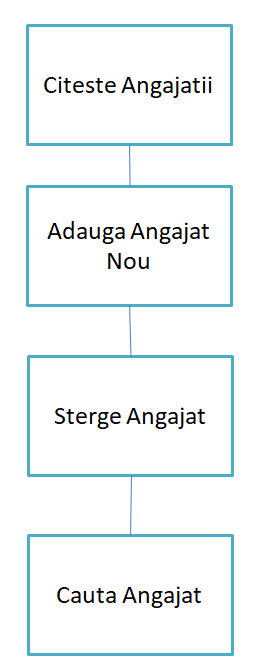
\includegraphics[width=7cm]{schema logica.png}
    \textbf{   \caption{Optiuni Meniu}}
    \label{fig:enter-label}
\end{figure}

\newpage 
\section{DESCRIEREA APLICATIEI}
\subsection{Utilizare}
Aplicația de management al angajaților este o unealtă simplă dezvoltată în limbajul C, care permite utilizatorilor să gestioneze informațiile despre angajați într-un mod interactiv. \\
\textbf{\textit{O scurtă descriere a utilizării aplicației:\\\\}}
\textbf{Lansarea Aplicației:\\}
Utilizatorul lansează aplicația de la consolă sau terminal.\\\\
\textbf{Afișarea Meniului:\\}
La început, aplicația afișează un meniu interactiv care oferă diferite opțiuni. Utilizatorul poate vedea tabelul cu angajați, adăuga un nou angajat, șterge un angajat, caută un angajat sau să iasă din aplicație.\\\\
\textbf{Afișarea Angajaților:\\}
Opțiunea "Afisati tabelul cu angajati" permite utilizatorului să vadă informațiile despre toți angajații existenți în sistem.\\\\
\textbf{Adăugarea unui Angajat Nou:\\}
Opțiunea "Adaugati o noua inregistrare" permite utilizatorului să introducă datele unui angajat nou, inclusiv ID-ul, numele și rolul.\\\\
\textbf{Ștergerea unui Angajat:\\}
Opțiunea "Stergeti o inregistrare" permite utilizatorului să șteargă un angajat existent în funcție de ID-ul acestuia.\\\\
\textbf{Căutarea unui Angajat:\\}
Opțiunea "Cautati o inregistrare" permite utilizatorului să introducă ID-ul unui angajat și să afle informațiile despre acel angajat.\\\\
\textbf{Ieșire din Aplicație:\\}
Opțiunea "Iesiti" încheie aplicația și închide meniul.\\\\
\textbf{Salvarea și Încărcarea Datelor:\\}
Datele angajaților sunt salvate într-un fișier la închiderea aplicației și încărcate din acel fișier la pornirea aplicației.\\\\
\textbf{Validări:\\}
Aplicația oferă feedback și mesaje de eroare pentru a asigura că utilizatorul introduce date valide și că operațiile sunt efectuate corect.\\\\
\textbf{Interacțiune Continuă:\\}
Utilizatorul poate interacționa cu aplicația într-un mod iterativ, efectuând diferite operații până când decide să iasă din aplicație.\\
Această aplicație simplă oferă un mediu interactiv pentru gestionarea datelor despre angajați și permite utilizatorilor să facă diverse operații asupra acestora.

\newpage

\subsection{Avantaje}
Utilizarea aplicației de management al angajaților dezvoltată în limbajul C oferă mai multe avantaje, în special pentru gestionarea și monitorizarea eficientă a informațiilor despre angajați într-o companie sau organizație. \\\\
\textbf{\textit{Câteva dintre avantajele utilizării acestei aplicații:\\\\}}
\textbf{Ușurința Utilizării:\\}
Interfața simplă și meniul interactiv fac aplicația ușor de utilizat, chiar și pentru persoanele fără experiență în programare.\\\\
\textbf{Gestionarea Eficientă a Angajaților:}
Utilizatorii pot adăuga, șterge, căuta și vizualiza informații despre angajați, facilitând gestionarea resurselor umane în organizație.\\\\
\textbf{\textit{Salvare și Încărcare Automată a Datelor:\\}}
Datele despre angajați sunt salvate automat la închiderea aplicației și încărcate la deschiderea acesteia, oferind consistență și persistență datelor.\\\\
\textbf{Rezolvarea Rapidă a Problemei:}
Utilizatorii pot identifica rapid angajați, adăuga noi informații sau șterge datele existente, rezolvând rapid problemele legate de informațiile despre angajați.\\\\
\textbf{Feedback și Validare:\\}
Aplicația oferă feedback utilizatorului și validează datele introduse, asigurându-se că acestea sunt corecte și complete.\\\\
\textbf{Automatizarea Proceselor Repetitive:\\}
Aplicația permite automatizarea unor procese repetitive legate de gestionarea angajaților, cum ar fi adăugarea sau ștergerea acestora.\\\\
\textbf{Portabilitate și Accesibilitate:\\}
Dezvoltată în limbajul C, aplicația poate fi compilată și rulată pe diverse platforme, oferind portabilitate și accesibilitate.\\\\
\textbf{Personalizare Ușoară:\\}
Utilizatorii pot modifica ușor codul sursă pentru a adăuga funcționalități suplimentare sau pentru a personaliza aplicația în funcție de nevoile specifice ale organizației.\\\\
\textbf{Învățare și Dezvoltare:\\}
Aplicația oferă o oportunitate pentru cei care doresc să învețe sau să dezvolte abilități în programare în limbajul C.\\\\
\textbf{Flexibilitate în Utilizare:\\}
Utilizatorii pot executa diferite operații într-o ordine flexibilă, adaptând aplicația la nevoile lor specifice.\\\\

\newpage

\subsection{Dezavantaje}
Deși aplicația de management al angajaților dezvoltată în limbajul C are numeroase avantaje, există și câteva dezavantaje, cum ar fi:\\\\
\textbf{Interfață Textuală:\\}
Interfața text-based poate să nu fie la fel de atrăgătoare sau intuitivă pentru toți utilizatorii, în special pentru cei obișnuiți cu aplicații grafice.\\\\
\textbf{Limitări în Extensibilitate:\\}
Extinderea funcționalității sau adăugarea de caracteristici noi poate fi mai dificilă în comparație cu aplicațiile dezvoltate în limbaje mai moderne și orientate pe obiect.\\\\
\textbf{Gestionare Manuală a Fișierelor:\\}
Aplicația salvează și încarcă datele în mod manual dintr-un fișier text, ceea ce poate fi nepractic într-un mediu unde gestionarea datelor se face în baze de date mai avansate.\\\\
\textbf{Lipsa Securității Avansate:\\}
Aplicația nu dispune de caracteristici avansate de securitate, cum ar fi autentificarea utilizatorilor sau criptarea datelor, ceea ce poate fi o vulnerabilitate în medii sensibile.\\\\
\textbf{Limitări în Manipularea Datelor:\\}
Manipularea datelor este limitată la operațiuni de bază (adică adăugare, ștergere, căutare), iar operațiuni complexe sau filtrare avansată pot să lipsească.\\\\
\textbf{Dependență de Cunoștințe Tehnice:\\}
Utilizarea eficientă a aplicației poate necesita cunoștințe minime de programare în limbajul C, ceea ce poate exclude anumite categorii de utilizatori.\\\\
\textbf{Lipsa Interactivității Avansate:\\}
Nu oferă funcționalități interactive avansate sau interfețe grafice, ceea ce poate limita experiența utilizatorului în comparație cu aplicațiile moderne.\\\\
\textbf{Gestionarea Manuală a Memoriei:\\}
Dezvoltarea în limbajul C implică gestionarea manuală a memoriei, ceea ce poate duce la posibile erori de memorie sau scurgeri dacă nu este gestionată corespunzător.\\\\


\section{REZULTATE}
Utilizatorii pot efectua o varietate de operațiuni asupra acestor date, inclusiv vizualizarea și actualizarea tabelului cu angajați, adăugarea unor noi intrări, ștergerea sau căutarea de înregistrări specifice. Astfel, oferă un mediu practic și accesibil pentru administrarea eficientă a detaliilor legate de personal în cadrul unei organizații.\\\\
Figura următoare arată meniul cu opțiunile disponibile și fișierul ce conține datele introduse de către utilizator:

\begin{figure}
    \centering
    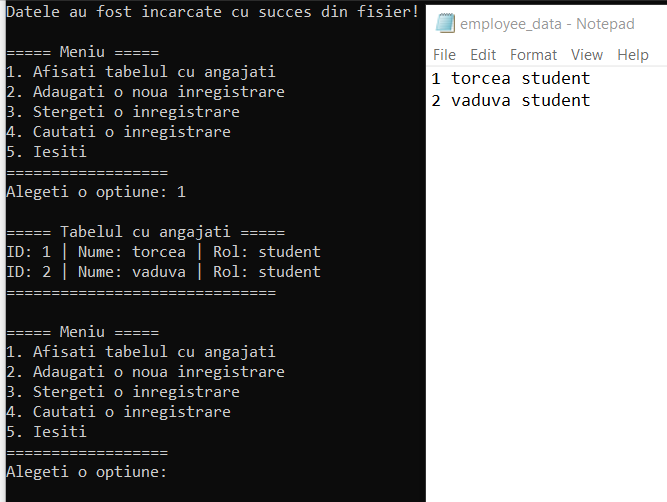
\includegraphics[width=17cm]{rezultate.png}
    \textbf{   \caption{Inserare și afișare date angajați}}
    \label{fig:enter-label}
\end{figure}

\newpage
\section{CONCLUZII}

În urma dezvoltării acestei aplicații simple de management al angajaților în limbajul C, putem trage câteva concluzii relevante:\\\\
\textbf{Simplu și Eficient:\\}
Aplicația oferă o soluție simplă și eficientă pentru gestionarea informațiilor despre angajați, utilizând un limbaj de programare precum C.\\\\
\textbf{Structură Modulară:\\}
Implementarea modulară, cu funcții dedicate pentru fiecare operațiune, facilitează înțelegerea și întreținerea codului.\\\\
\textbf{Interactivitate:\\}
Meniul interactiv permite utilizatorilor să interacționeze ușor cu aplicația, efectuând diverse operațiuni asupra datelor despre angajați.\\\\
\textbf{Persistența Datelor:\\}
Salvarea și încărcarea automată a datelor într-un fișier text asigură persistența informațiilor între diferite rulări ale aplicației.\\\\
\textbf{Limitări și Dezavantaje:\\}
Totuși, aplicația are și limitările sale, cum ar fi lipsa caracteristicilor avansate și a interfeței grafice.\\\\

\section{APPENDIX: PROGRAM C}

\lstinputlisting{main.c}

\section{BIBLIOGRAFIE}
% bibliography
\begin{thebibliography}{9}
\label{sec_ref}
\bibitem{overleaf-doc}
    Overleaf Documentation,\urlstyle{same} {\small \url{https://www.overleaf.com/learn}}. 
\bibitem{overleaf-tutorials}
    Overleaf Turotials,\urlstyle{same} {\small \url{https://www.overleaf.com/learn/latex/Tutorials}}. 
\bibitem{employee-management}
   Employee Management System Project using C,\urlstyle{same} {\small \url{https://www.studytonight.com/c-projects/employee-management-system-project-using-c-language}}. 
\bibitem{employee-record}
   Employee Record System in C using File Handling,\urlstyle{same} {\small \url{https://www.geeksforgeeks.org/employee-record-system-in-c-using-file-handling/}}. 
\bibitem{c-tutorials}
   C Tutorials,\urlstyle{same} {\small \url{https://www.w3schools.com/c/}}. 
\bibitem{menu}
    Menu-Driven program using Switch-case in C,\urlstyle{same} {\small \url{https://www.geeksforgeeks.org/menu-driven-program-using-switch-case-c/}}. 
    
\end{thebibliography}



\end{document}